对于有许多条件语句(通常是\texttt{if()}语句)的程序,分支预测的有效性通常决定了整体性能。如果准确地预测分支,那么在分支上基本上没有任何开销。要是分支预测有一半是错误的,可能会比常规算术指令慢十倍或更多。

硬件分支预测是基于处理器执行的条件指令。因此,处理器对条件的理解可能与我们不同。下面的例子有助于我们理解这一点:

\hspace*{\fill} \\ %插入空行
\noindent
\textbf{02\_branch.C}
\begin{lstlisting}[style=styleCXX]
std::vector<unsigned long> v1(N), v2(N);
std::vector<int> c1(N), c2(N);
for (size_t i = 0; i < N; ++i) {
	v1[i] = rand();
	v2[i] = rand();
	c1[i] = rand() & 0x1;
	c2[i] = !c1[i];
}
unsigned long* p1 = v1.data();
unsigned long* p2 = v2.data();
int* b1 = c1.data();
int* b2 = c2.data();
for (auto _ : state) {
	unsigned long a1 = 0, a2 = 0;
	for (size_t i = 0; i < N; ++i) {
		if (b1[i] || b2[i]) { // !!!
			a1 += p1[i];
		} else {
			a1 *= p2[i];
		}
	}
	benchmark::DoNotOptimize(a1);
	benchmark::DoNotOptimize(a2);
	benchmark::ClobberMemory();
}
\end{lstlisting}

有趣的是\texttt{if (b1[i] || b2[i])}条件:计算总为\texttt{true},因此可以期待处理器的完美预测。当然,事情没这么简单。从逻辑上,看起来这一个单独的条件,但对从CPU角度来说,是两个独立的条件分支:一半的情况下,在第一个分支,总体结果正确;另一半情况下,使它正确的是第二个分支。结果总的是正确的,但不可能预测哪个分支是正确的。

%\hspace*{\fill} \\ %插入空行
\begin{center}
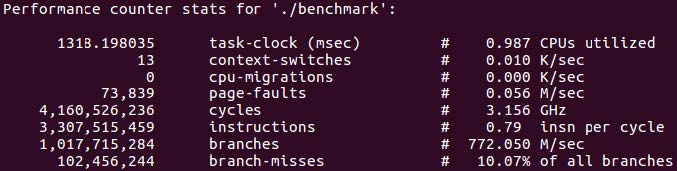
\includegraphics[width=0.9\textwidth]{content/1/chapter3/images/27.jpg}\\
图3.27 - “假”分支的分支预测
\end{center}

分析器显示与真正随机分支一样差的分支预测率。性能基准测试结果更证实了我们的猜想:

%\hspace*{\fill} \\ %插入空行
\begin{center}
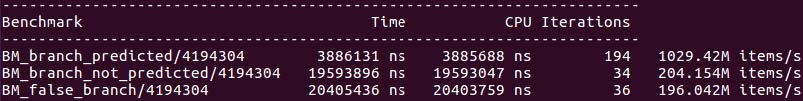
\includegraphics[width=0.9\textwidth]{content/1/chapter3/images/28.jpg}\\
图 3.28
\end{center}

\textit{假}分支(不是真正的分支)的性能与真正随机的、不可预测的分支一样糟糕。

实际程序中,不应该出现这种不必要的条件语句。然而,常见的是复杂的条件表达式,其计算结果几乎相同。例如,可能有一个条件很少为\texttt{false}:

\begin{lstlisting}[style=styleCXX]
if ((c1 && c2) || c3) {
	… true branch …
} else {
	… false branch …
}
\end{lstlisting}

几乎一半的情况\texttt{c3}都是\texttt{true}。当\texttt{c3}为\texttt{false}时,\texttt{c1}和\texttt{c2}通常都为\texttt{true}。总条件应该容易预测,并且采用真分支。从处理器的角度来看,它不是一个单独的条件,而是三个单独的条件跳跃。如果\texttt{c1}为\texttt{true},那么必须检查\texttt{c2}。如果\texttt{c2}也为\texttt{true},则执行跳转到真分支的第一个指令。如果\texttt{c1}或\texttt{c2}中的一个为\texttt{false},则检查\texttt{c3}。如果为\texttt{true},则执行再次跳转到\texttt{true}分支。

这个求值必须按特定顺序完成,C++标准(以及在此之前的C标准)规定,像\&\&和||这样的逻辑操作可以短路。当整个表达式的结果已知,对表达式其余部分的计算就应该停止。这在条件语句具有有副作用时尤为重要:

\begin{lstlisting}[style=styleCXX]
if (f1() || f2()) {
	… true branch …
} else {
	… false branch …
}
\end{lstlisting}

只有当\texttt{f1()}返回\texttt{false}时,才会调用函数\texttt{f2()}。前面的例子中,条件是简单的布尔变量\texttt{c1}、\texttt{c2}和\texttt{c3}。编译器已经知道没有任何副作用,并且计算整个表达式不会改变可观察行为。有些编译器会做这种优化。如果\textit{假分支}基准测试使用这样的编译器,则会有良好的分支预测性能。但多数编译器并没有意识到这是一个问题(事实上,编译器没有办法知道整个表达式的计算结果常为\texttt{true})。因此,这个优化需要开发手动完成。

假设开发者知道\texttt{if()}的两个分支中有一个经常使用,例如:\texttt{else}分支可以对应错误情况,或其他一些必须正确处理,但在正常操作下不应出现的异常情况。假设做了正确的事情,并使用分析器进行了验证,组成复杂布尔表达式的单个条件指令并没有得到很好的预测。这时,如何优化代码?

第一件事可能是将条件求值移出\texttt{if()}语句:

\begin{lstlisting}[style=styleCXX]
const bool c = (c1 && c2) || c3;
if (c) { … } else { … }
\end{lstlisting}

这肯定不会奏效,原因有二。首先,条件表达式使用逻辑\&\&和||操作,因此计算会短路,并且需要单独和不可预测的分支。其次,编译器可能会通过删除不必要的临时变量\texttt{c}来优化这段代码,因此最终的代码可能根本不会改变。

对条件变量数组进行循环时,可以使用类似的转换。下面这段代码很可能会受到分支预测的影响:

\begin{lstlisting}[style=styleCXX]
for (size_i i = 0; i < N; ++i) {
	if ((c1[i] && c2[i]) || c3[i]) { … } else { … }
}
\end{lstlisting}

但是,如果预先计算所有的条件表达式,并存储在一个新数组中,大多数编译器都不会干掉这个临时数组:

\begin{lstlisting}[style=styleCXX]
for (size_i i = 0; i < N; ++i) {
	c[i] = (c1[i] && c2[i]) || c3[i];
}
…
for (size_i i = 0; i < N; ++i) {
	if (c[i]) { … } else { … }
}
\end{lstlisting}

当然,用于初始化\texttt{c[i]}的布尔表达式,现在面临着分支预测错误的问题,因此只有当第二个循环执行的次数比初始化循环多很多时,这种转换才会有用。

通常有效的优化方法是用加法和乘法,或按位\&和|操作替换逻辑\&\&和||操作。这样做之前,必须确定\&\&和||操作的参数是布尔值(值为0或1)而不是整数。即使值2解释为真,表达式\texttt{2 \& 1}的结果与\texttt{bool(2) \& bool(1)}的结果也不相同。前者的计算结果为0(\texttt{false}),而后者预期的正确答案为1(或\texttt{true})。

我们可以在基准测试中比较这些优化代码的性能:

%\hspace*{\fill} \\ %插入空行
\begin{center}
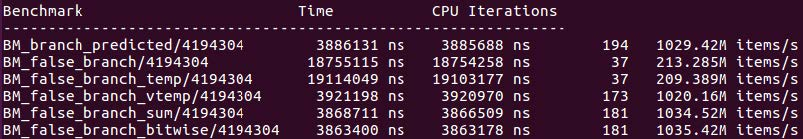
\includegraphics[width=0.9\textwidth]{content/1/chapter3/images/29.jpg}\\
图 3.29
\end{center}

通过引入临时变量\texttt{BM\_false\_branch\_temp}来优化\textit{假分支}的尝试完全没有效果。因为临时向量的所有元素都为\texttt{true},这就是分支预测器所知道的(\texttt{BM\_false\_branch\_vtemp}),所以临时向量给出了一个完全预测的分支的预期性能。用算术加法(+)或按位|替换逻辑||会产生类似的结果。

最后两个转换(使用算术或位操作,而不是逻辑操作)改变了代码的含义:表达式中所有操作的参数都是求值的,并具有副作用。由编程者决定此更改是否会影响程序的正确性。如果副作用开销特别大,那么总体性能收益会是负的,例如:如果\texttt{f1()}和\texttt{f2()}非常耗时,那么用等价的算术加法(\texttt{f1() + f2()})替换表达式\texttt{f1()|| f2()}中的操作会让性能下降(即使它改善了分支预测)。

总的来说,没有标准的方法来优化\textit{假分支}中的分支预测,这就是为什么编译器难进行有效的优化。开发者必须使用特定于问题的知识,例如:某个特定条件是否可能发生,并将其与分析结果相结合,以获得最佳的解决方案。

了解了CPU操作如何影响性能,然后扩展到一个具体的和实际相关的例子中,并将这些知识应用于代码优化。在结束本章之前,再来看一个优化示例。



























